\begin{figure}
    \centering
    \begin{subfigure}{0.48\textwidth}
        \centering
        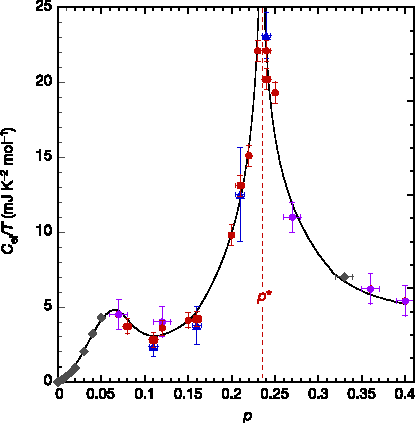
\includegraphics[width=\textwidth]{figures/michon}
        \caption{Michon et al.\cite{michon2019}}
        \label{fig:michon}
    \end{subfigure}\hfill
    \begin{subfigure}{0.48\textwidth}
        \centering
        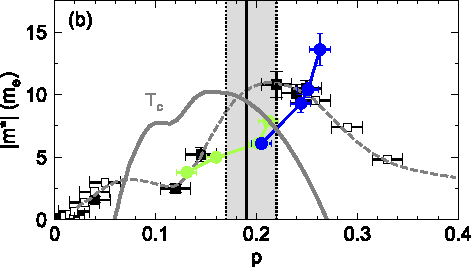
\includegraphics[width=\textwidth]{figures/legros}
        \caption{Legros et al.\cite{legros2022}}
        \label{fig:legros}
    \end{subfigure}
    \caption{Comparison of the measurements of Michon et al.\cite{michon2019} and Legros et al.\cite{legros2022} In (a), measurements
    of Michon et al. showing a peak in $C/T$ which signifies the existence of a QCP. In (b),
    measurements of Legros et al. drawn onto the measurements from Michon et al.,
    showing no peak in the cyclotron mass.}
    \label{fig:comparison}
\end{figure}

\subsection{Evidence against the QCP: Optical Conductivity}
In their 2022 paper, Legros et al.\cite{legros2022} instead used optical conductivity to
probe the QCP. To do so, they first measured the optical conductivity of LSCO cuprates\footnote{
LSCO is a cuprate with the formula La$_{2-x}$Sr$_x$CuO$_4$, where $x$ indicates the doping level.} in various fields. 
Then, they fitted a model the data. 
The Drude formula which they used, is a simple classical model that has been used for a long time in condensed matter physics to model conductivity. 
With this, they extracted the cyclotron mass $m_c$ from the parameters of the fit.

They argued the cyclotron mass is the same as the effective mass of the charge carriers
($m_c \sim m^*$), which is not rigorously true and can be a good or bad approximation depending on the case.

At the end of all the analysis, Legros et al.\cite{legros2022} found that the cyclotron mass does not peak
at the critical doping level and simply increases with doping (Figure \ref{fig:legros}). This is in contradiction with the
results of Michon et al. and suggests that there is no QCP in cuprates.

We believe, however, that their data analysis is problematic, because of their choice of model. 
The Drude formula, derived using classical physics, is highly effective for
analyzing the conductivity of materials, which emerges from the collective quantum behavior of the
electrons\footnote{more precisely, the Fermi surface needs to be approximately isotropic}. 
But, this is not true for cuprates, 
which have highly anisotropic electronic properties.\footnote{See Figure
\ref{fig:fermi_surface}. The Fermi surface is not anisotropic at all, and there is no reasonable
approximation for interpreting it in a roughly isotropic way.} 
One can also question the validity of the approximation that $m_c \sim m^*$, 
however this was not a focus of our project.
